\begin{figure*}[ht!]
  \centering
  \vspace{-2.6cm}
  \centerline{
    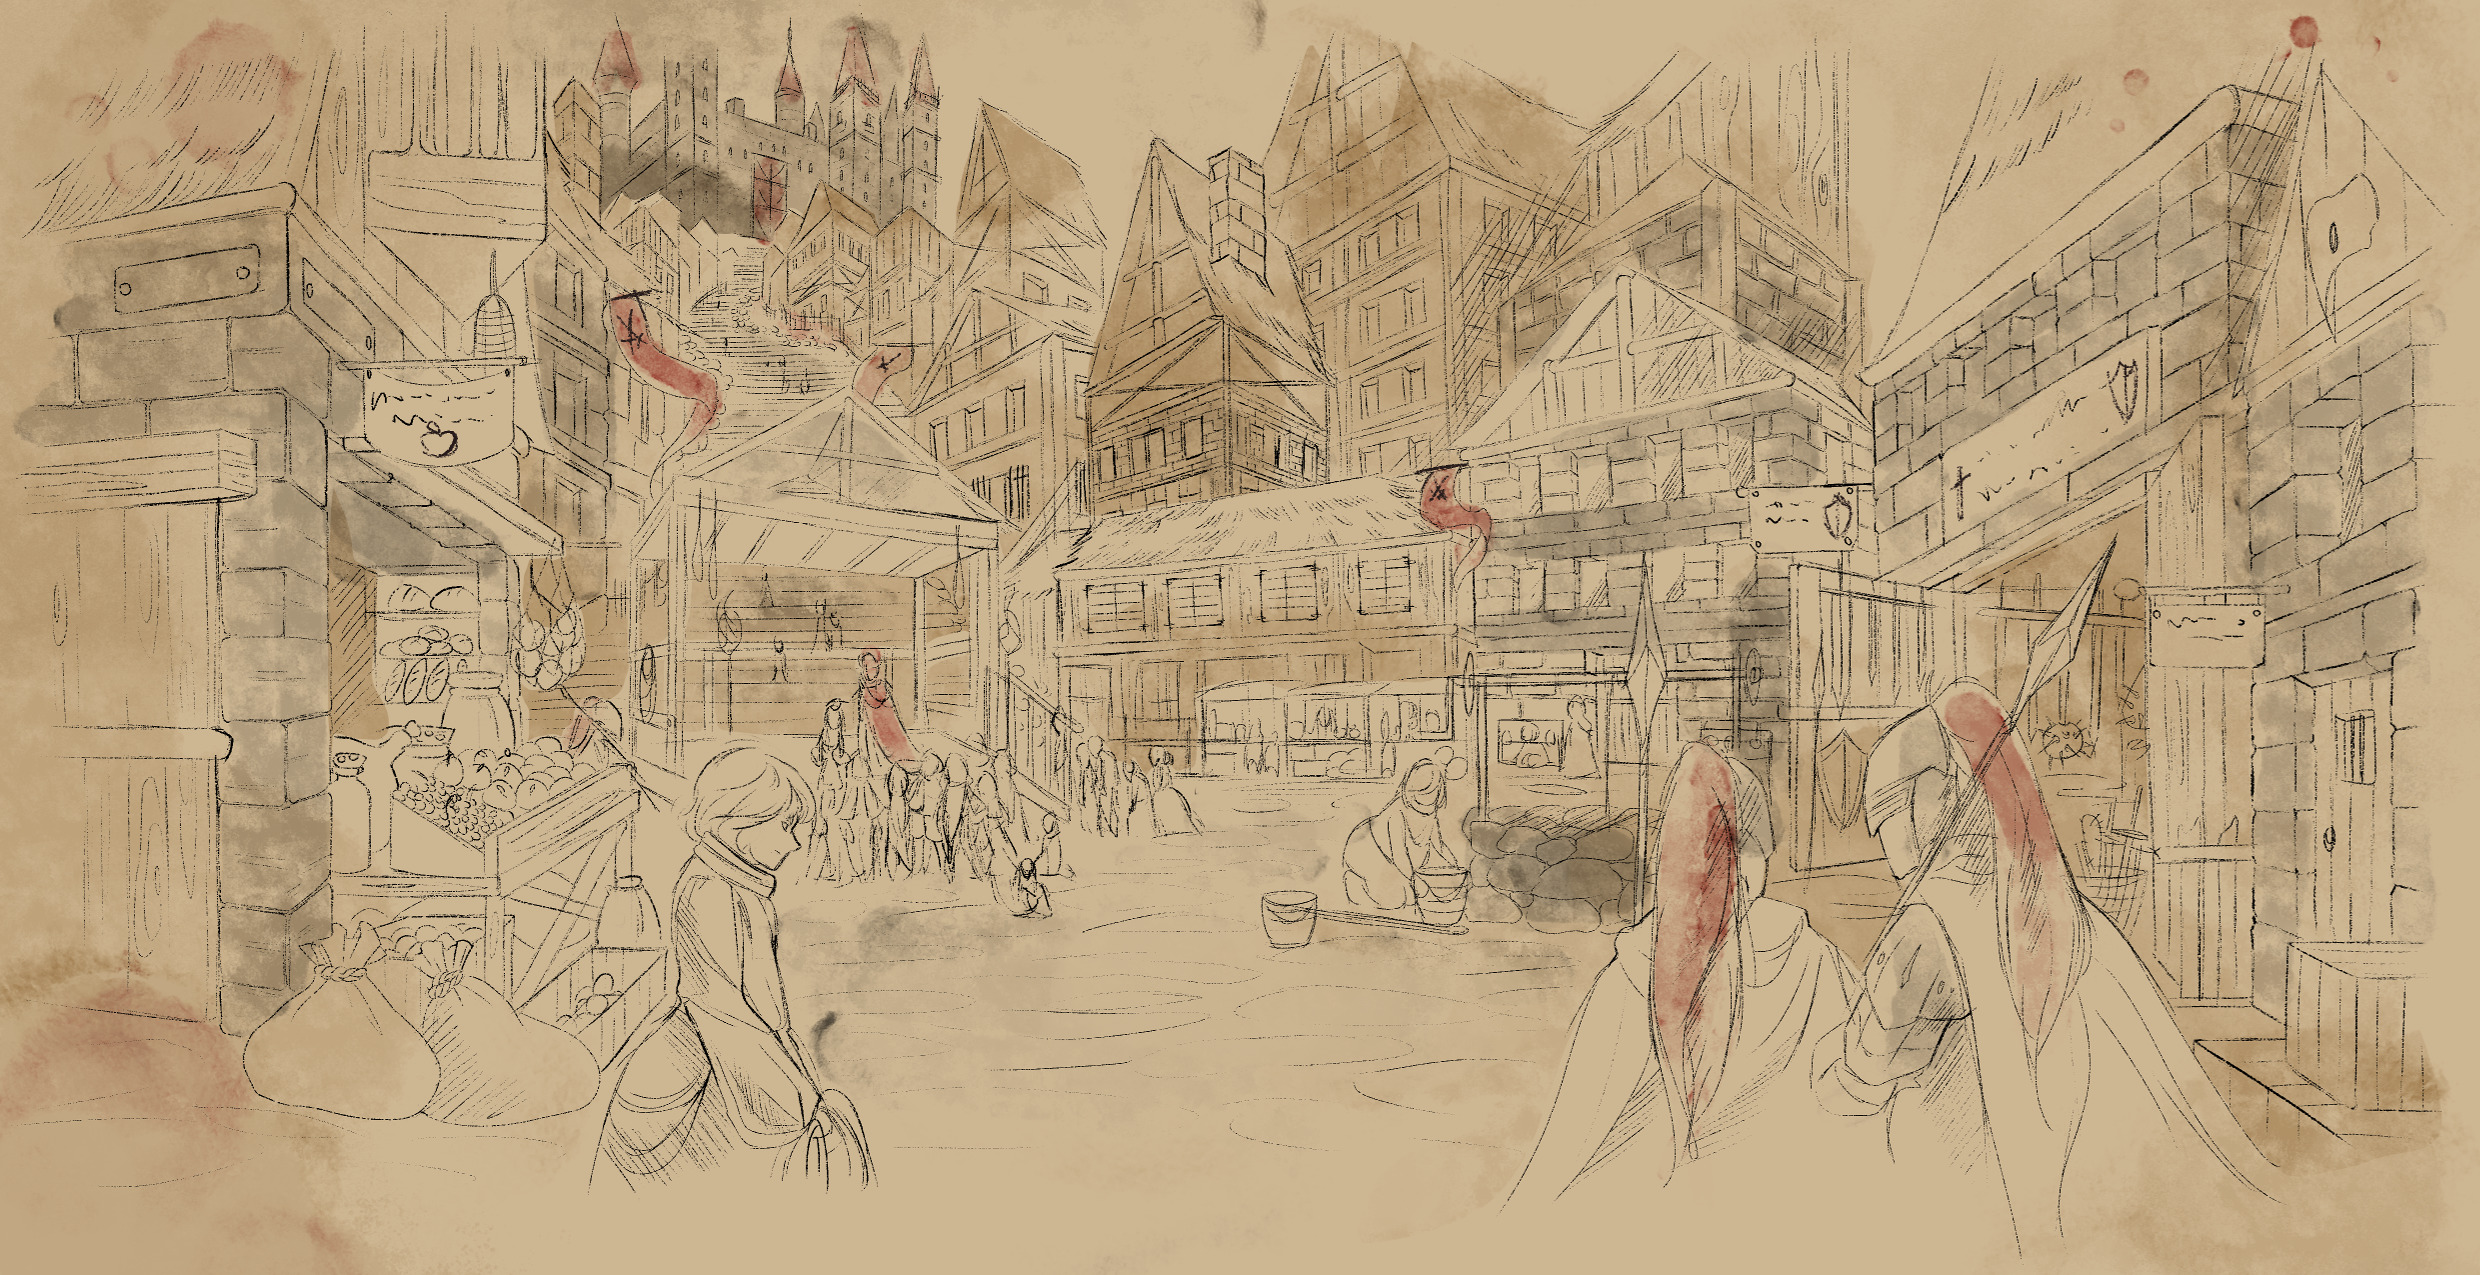
\includegraphics[width=\paperwidth,keepaspectratio]{media/norburysm.png}
  }
  \par
  Market place in \emph{Norbury}, circa GT:2102
\end{figure*}

\subsection{Norbury}
\label{sec:Norbury}

\graham{Surely the most vile city kingdom Aror has to offer...}
\aren{Bless thy innocent heart, for you have not lived long enough to see the
  rise of Morkan.}

The second youngest city kingdom, \emph{Norbury} resides on a large island off
the northern coast of the continent \emph{Eilean Mor}. Norbury is a large
walled city, encompassing a quarter of the huge island.

\subsubsection{History}

It was founded around \emph{GT:1849} as a joint military outpost of
\emph{Hraglund} and other northern baronies of Eilean Mor. It was originally
founded as first line of defence against the many raids of the beast races
that came from the northern most continent of \emph{Iâfandir}. Quickly the
fortress of Norbury grew into a castle, and more and more people were
required to keep the castle and its army supplied. Armies need smiths,
smiths need smelters, smelters need coal huts and miners, and all of
these need food, lodging and entertainment. Within a few generations
Norbury exploded in size and population, all working towards one goal:
keeping the raids and incursion of the beast races away from the main
continent.

\subsubsection{Banner}

\begin{figure}[!ht]
  \centering
  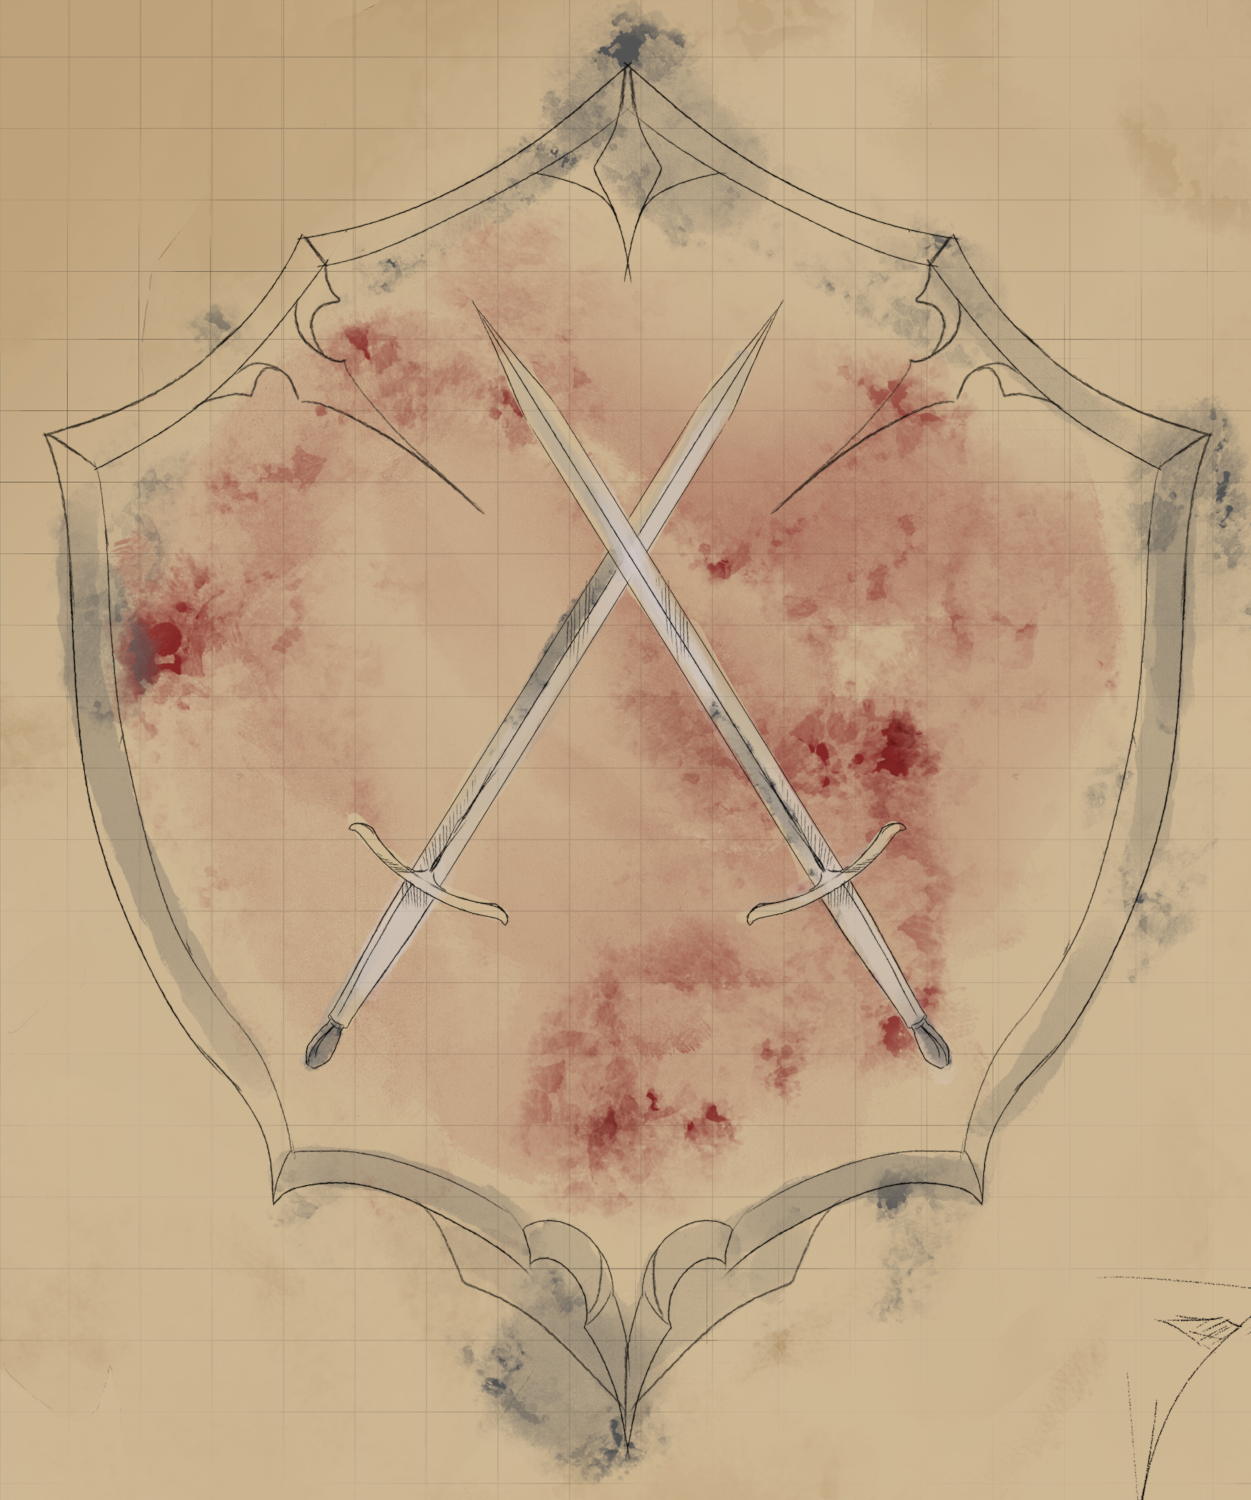
\includegraphics[width=0.9\linewidth]{media/norbury-bannersm.png}
\end{figure}

The kingdom's banner shows two silver swords crossed at the blade, against a
light red background. The main colours of the kingdom are silver and red.

\subsubsection{Districts}

The centre of the city is a large market place, with a big stone steeple in
the middle. The tower both signifies the eternal vigilance, but also houses a
large bell that is rung in case of an attack. Inscribed into the walls of
the steeple are the laws of the kingdom for everybody to read. The market
place is vast circular open courtyard, and all sorts of goods - including
slaves - are sold there.

To the north lies \emph{Norbury} castle, a huge fortified military camp and
seat of the monarch. It oversees the northern sea off the island, and rests
upon a roughly two hundred metre high cliff side.

The surrounding area of the walled city houses farms and smaller villages that
are ruled by the kingdom as well. Since these farms are exposed to sea raids,
the northern shores of the island are dotted with small military camps, guard
towers and outlooks that notify the villages of impending raids.

\subsubsection{Sea Raids}

A network of watch towers, light houses, guard towers and scout ships
constantly check the sea north of \nameref{sec:Eilean Mor} for any impending
sea raiders that embark from the continent of \nameref{sec:Iafandir}. If a
suspicious ship or raiding party is discovered, the entire kingdom goes on
high alert and deploys their fleet. Norbury are excellent ship builders,
sailors and warriors on the sea; and so they prefer to capture and destroy
raiding parties before they land on Eilean Mor. Most of the ships manned by
the beast races of \nameref{sec:Iafandir} are often inferior and incapable of
prolonged sea battle and thus are often sunk off the coast of the
continent. The raiders that survive are fished out of the sea and then brought
back to Norbury as slaves.

Sometimes raiding parties do sneak past the ever vigilant eye of the city,
and then land on the northern shores of Eilean Mor. Most of the baronies
on the shores have increased their armies to repel these raids upon their
lands. Yet some also call the mainstay army of Norbury for aid. Then the
soldiers of the barony bars the raiders from entering their land, while the
ships and navy of Norbury attack the landing party from the sea.

Defending Eilean Mor (the ``home land'') from sea raids is a cultural goal and
ideal, that is extended to any barony on the main continent. Some warriors of
Norbury even see it as impolite to ask for compensation or gold in exchange,
as there is enough honour already in defending their brethren of the main
land. Still many baronies and smaller earldoms pay Norbury for their aid,
either in gold, everblack or in trade deals highly favouring Norbury.

\subsubsection{Religious Civil War}
\label{sec:Religious Civil War}

Ever since its foundation, the religions surrounding \nameref{sec:Lor}, the
\nameref{sec:Order} and the \nameref{sec:Three Kings} vied for the position of
dominance within the city. The Order had the most followers, followed by Three
Kings and then Lor. Although the priests and paladins of Order raised issues
with mistreatment of slaves, they were not outright against slavery, unlike
the priests and followers of Lor who wished to see the practice banned. The
followers of the Three Kings found both the followers of Lor and the Order to
be weak in the face of their common enemy from the north, and were ready to
expel both religions from the city. Over centuries this conflict hardened and
brewed in the heads of the followers and citizens. Then, in \emph{MI:1480}
when a follower of the Three Kings beat his slave to death with a pavement
stone in the middle of the market place for disobeying him, a paladin of Lor
interfered, killing the slave owner in single combat. This event brought a spark
to the already volatile mix of religious animosity. The followers of the Three
Kings moved in retaliation against the temple and followers of Lor. The
Order, who sided with the mistreated slave, joined the conflict on the side of
the followers of Lor. The civil war lasted for two weeks, in which both the
Order and the followers of Lor suffered heavy losses and ultimately defeat
against a force inferior in numbers. To prevent the bloodshed to spilling over
to civilians, the then ruling queen Arianna of Nordholm, banned the religions
associated with Lor and Order and exiled their followers for being ``weak in
the face of adversity''.

This conflict has long passed, but still the prevailing attitude in Norbury is
that followers of the Order and Lor were, and are still, weak and not worthy
of honour. Although the ban is still in place, the exile has since been
lifted, allowing priests and paladins of the two gods to visit the city.

\subsubsection{Culture}

Since the incursion and raids of the beast races still occur to this day,
and have grown to be more ferocious and demanding, the culture of Norbury
has grown in response. Norbury is from the lowliest slave and peasant up
to the king or queen herself, a meritocracy. You are worth as much to the
city and in the eyes of your fellow citizen as you can contribute to the
defence effort.

Men and women of Norbury pride themselves in the work they are contributing to
the collective defence effort, be it front line combat, creating weapons and
armour for those that do, or aiding the effort in an administrative
fashion. Warrior culture runs strong in the kingdom, their deeds are sung in
taverns, their likeness is made eternal in art. Many fighters and warriors of
Norbury follow the \emph{Three Kings}, although worship of \emph{Forun} is also
wide spread in the kingdom.

Although arcane and divine magic is still frowned upon in the kingdom, the army
of Norbury runs an academy for battle mages and wizards. Arcane research is
often scrutinized by its potential military application, and wizards are also
required to undergo basic military training in weapons and armour.

All citizens of Norbury (and those that wish to become citizens) must complete
a mandatory civil service of at least five years. Many use this mandatory
service to begin an apprenticeship, while others join the military and counter
raids. No one is excluded from this service, not even the children of the
reigning monarchs. Avoiding this service is seen as a great dishonour, and a
major crime.

\subsubsection{Society}

Titles within the kingdom's society, such as commoner, earl, baron or even
duke and grand duke can be bought by any citizen of Norbury. There is a rather
unusual twist: These titles are not inherited, which means that the son of a
duke is a commoner upon birth. The common census is, that this child has not
done anything yet to earn the rank of earl for him or herself. There is a high
pressure on children to achieve the same status as their parents, or perhaps
even outperform them. Failure is always an option as well, as it is not
unheard of for a noble son to fall into slavery.

Who reigns as king or queen is decided in a ritual combat between all eligible
arch dukes that wish to rise to the challenge. This combat is not to the
death, although many grand duke's have perished in their claim for the
kingdom. A king or queen reins until his reign is challenged by another, or
until they die or resign. The people of Norbury mostly do not care what race
or social background of their king or queen, but instead judge all their peers
by their honour, combat prowess, and contribution to society as a whole.

\subsubsection{Slavery}
\label{sec:Slavery in Norbury}

Norbury is the foremost kingdom to practice slavery on a massive scale. Both
\hyperref[sec:Indentured Servitude]{indentured servitude} and
\hyperref[sec:Unregulated Slavery]{chattel slavery} are encoded in Norbury
law.

Many of the raiders that are captured, and most of those that commit major
crimes are enslaved. The wizard academy as constructed special
\hyperref[sec:Slave Band]{arcane collars} that bind the slave to their
owners. Slavery is often a sentence for life, as there is no legal way to
escape slavery, unless the owner releases the slave. A legal hurdle that is
not cheap to the owner. Norbury slaves have no rights whatsoever, and are
marked, colour coded, registered by number, and tracked down by the
\nameref{sec:Hunters Guild} should they decide to run. Slave collars allow
their owners to track, command and often punish their wearers.

Foreigners are allowed to purchase slaves, however they have to pay an
additional fee half the slave's value. This was intentionally done, so that
most of the slaves remain within the city and contribute to the city. Slave
ownership is recognised as lawful in all kingdoms and baronies that have
signed the \hyperref[sec:Vonir Accord]{Vonir Accord}.

Although the city has a large slavery population (between 30 and 40 percent),
it rarely faces slave revolts or uprisings. There are four main pacifiers at
work, that keep the slave population suppressed and obedient. First, for many
slavery is potentially only temporary. Many join the Norbury army, the
Hunter's Guild or begin work in other positions that would qualify them for
citizenship later on, and thus do not wish to risk their permanent freedom
through revolt. The second is a ever permeating culture of honour and duty,
especially in the still ongoing sea raids from the north. Many slaves derive a
sense of purpose from working toward a common goal. Also many churches and
charitable organisations provide a network of services and goods, such as
food, warmth and medical services to slaves making their lives bearable.
Although gatherings of slaves are forbidden, the Hunter's Guild often looks
the other way in regard to slave bars or inns, as long as no direct threat
stems from these establishment. And the fourth reason is the ever vigilant
\nameref{sec:Hunters Guild}. Their network of informants, hunters and agents
quench any rebellious flame that might kindle in the dark.

\subsubsection{Population}

Norbury, and its outlying villages, houses roughly 4 million people. Of which
the vast majority are human and deepkin (39\%), then elves (24\%) followed by
dwarves (15\%) and half races (10\%). The rest (12\%) are beast races, almost
all of which are enslaved. Roughly 41\% of the entire population is either
currently enslaved or in servitude.
